\documentclass[11pt,a4paper]{article}

\usepackage[utf8]{inputenc}
\usepackage[T1]{fontenc}
\usepackage{lmodern}
\usepackage[margin=0.72in]{geometry}
\usepackage[table]{xcolor}
\usepackage{array}
\usepackage{tabularx}
\usepackage{booktabs}
\usepackage{enumitem}
\usepackage{titlesec}
\usepackage{fancyhdr}
\usepackage{lastpage}
\usepackage[hidelinks]{hyperref}
\usepackage{tikz}

\definecolor{TextInk}{HTML}{111111}
\definecolor{RuleGray}{HTML}{D9D9D9}
\definecolor{GraphDark}{gray}{0.28}
\definecolor{GraphMid}{gray}{0.58}
\definecolor{GraphLight}{gray}{0.82}

\hypersetup{
  pdftitle={Geography Standard Level Paper 1 Practice Simulation Set 2 - 2026-05-07},
  pdfauthor={IB Geography SL Preparation}
}

\color{TextInk}
\setlength{\parskip}{0.35em}
\setlength{\parindent}{0pt}
\setlength{\tabcolsep}{5pt}
\renewcommand{\arraystretch}{1.15}
\setlist[itemize]{leftmargin=1.45em,itemsep=3pt,topsep=4pt,label=\textbullet}

\newcolumntype{Y}{>{\raggedright\arraybackslash}X}
\newcolumntype{L}[1]{>{\raggedright\arraybackslash}p{#1}}

\titleformat{\section}
  {\normalfont\large\bfseries}
  {}{0pt}{}
\titleformat{\subsection}
  {\normalfont\normalsize\bfseries}
  {}{0pt}{}

\pagestyle{fancy}
\setlength{\headheight}{14pt}
\fancyhf{}
\fancyhead[C]{-- \thepage\ --}
\fancyhead[R]{Practice}
\renewcommand{\headrulewidth}{0pt}
\renewcommand{\footrulewidth}{0pt}

\newcommand{\markpts}[1]{\hfill\textbf{[#1]}}
\newcommand{\exam}[1]{#1}

\begin{document}

\thispagestyle{empty}
\begin{center}
{\Large Geography}\\[0.35em]
Standard level\\[0.35em]
Paper 1\\[1.8em]
7 May 2026\\[1.8em]
1 hour 30 minutes\\[2.8em]
Practice simulation set 2
\end{center}

\vspace{1.4em}

\textbf{Instructions to candidates}
\begin{itemize}
  \item Do not open this examination paper until instructed to do so.
  \item Answer the questions in two options.
  \item When relevant, answers should refer to case studies or examples, and
  where appropriate include well-drawn maps or diagrams.
  \item The maximum mark for this examination paper is \textbf{[40 marks]}.
\end{itemize}

\vspace{1.2em}

\begin{center}
\begin{tabular}{L{0.48\textwidth}L{0.22\textwidth}}
\toprule
\textbf{Option} & \textbf{Questions} \\
\midrule
Option F -- Food and health & 11--12 \\
Option G -- Urban environments & 13--14 \\
\bottomrule
\end{tabular}
\end{center}

\vfill
\noindent 5 pages \hfill Practice simulation

\newpage

\section{Option F -- Food and health}

\textbf{Answer the following question.}

\subsection{11.}

The graph shows three food and health indicators for four regions of a country
in the year following an extended dry season and a sharp rise in food prices.

\begin{center}
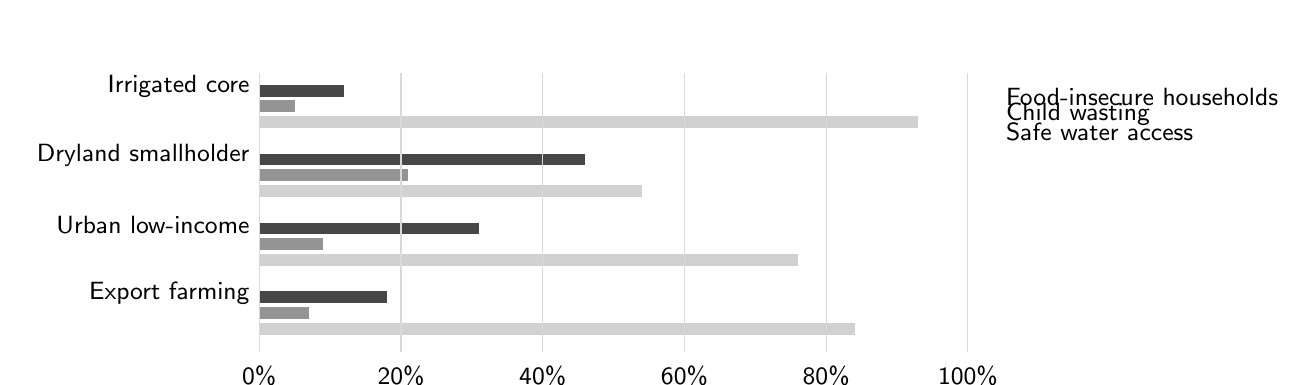
\begin{tikzpicture}[x=0.09cm,y=0.5cm, every node/.style={font=\sffamily\small}]
  \node[anchor=east] at (0,8.1) {Irrigated core};
  \draw[fill=GraphDark, draw=none] (0,7.85) rectangle (12,8.15);
  \draw[fill=GraphMid, draw=none] (0,7.45) rectangle (5,7.75);
  \draw[fill=GraphLight, draw=none] (0,7.05) rectangle (93,7.35);
  \node[anchor=east] at (0,6.35) {Dryland smallholder};
  \draw[fill=GraphDark, draw=none] (0,6.10) rectangle (46,6.40);
  \draw[fill=GraphMid, draw=none] (0,5.70) rectangle (21,6.00);
  \draw[fill=GraphLight, draw=none] (0,5.30) rectangle (54,5.60);
  \node[anchor=east] at (0,4.60) {Urban low-income};
  \draw[fill=GraphDark, draw=none] (0,4.35) rectangle (31,4.65);
  \draw[fill=GraphMid, draw=none] (0,3.95) rectangle (9,4.25);
  \draw[fill=GraphLight, draw=none] (0,3.55) rectangle (76,3.85);
  \node[anchor=east] at (0,2.85) {Export farming};
  \draw[fill=GraphDark, draw=none] (0,2.60) rectangle (18,2.90);
  \draw[fill=GraphMid, draw=none] (0,2.20) rectangle (7,2.50);
  \draw[fill=GraphLight, draw=none] (0,1.80) rectangle (84,2.10);
  \foreach \x in {0,20,40,60,80,100} {
    \draw[RuleGray] (\x,1.35) -- (\x,8.45);
    \node[anchor=north] at (\x,1.25) {\x\%};
  }
  \node[anchor=west] at (104,7.85) {Food-insecure households};
  \node[anchor=west] at (104,7.4) {Child wasting};
  \node[anchor=west] at (104,6.95) {Safe water access};
\end{tikzpicture}
\end{center}

\medskip

\noindent\textbf{(a)\ \ (i)}~\exam{Identify} the region with the highest
percentage of food-insecure households.\markpts{1}

\medskip
\noindent\hphantom{\textbf{(a)\ \ }}\textbf{(ii)}~\exam{State} the percentage of
households reporting child wasting in the dryland smallholder
region.\markpts{1}

\medskip
\noindent\textbf{(b)}~\exam{Outline} one way in which an extended dry season can
reduce safe water access in rural communities.\markpts{2}

\medskip
\noindent\textbf{(c)}~\exam{Explain} how a climate shock can lead to changes
in:

\medskip
\noindent\hphantom{\textbf{(c)}~}\textbf{(i)} child wasting in vulnerable rural
households;\markpts{3}

\medskip
\noindent\hphantom{\textbf{(c)}~}\textbf{(ii)} food prices in urban low-income
districts.\markpts{3}

\vspace{0.6em}
\textit{(Option F continues on the following page)}

\newpage

\textit{(Option F continued)}

\textbf{Answer either part (a) or part (b).}

\medskip
\noindent\textbf{Either}

\medskip
\noindent\textbf{12.\ (a)}~Using one or more named places, \exam{examine} the
links between malnutrition and infectious disease.\markpts{10}

\medskip
\noindent\textbf{Or}

\medskip
\noindent\textbf{12.\ (b)}~\exam{Evaluate} the success of strategies used to
improve food security following an environmental shock.\markpts{10}

\vspace{0.8em}
\textit{End of Option F}

\newpage

\section{Option G -- Urban environments}

\textbf{Answer the following question.}

\subsection{13.}

The graph shows the share of daily trips made by walking or cycling, public
transport, and private car in four zones of a large city. Each row sums to
100\%.

\begin{center}
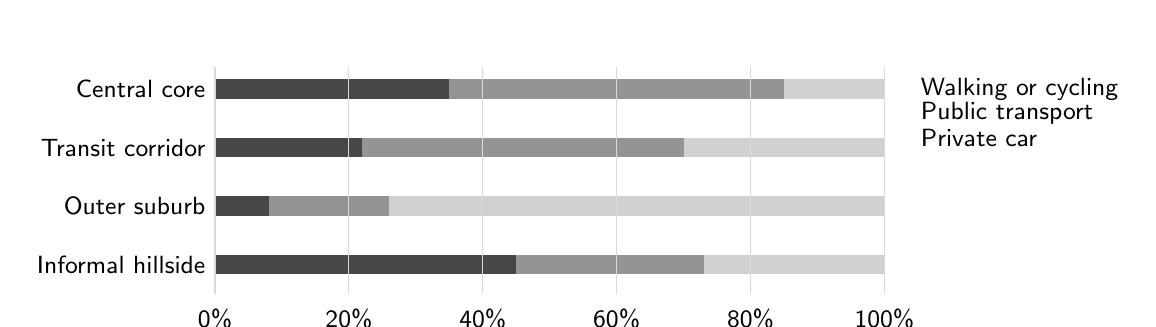
\begin{tikzpicture}[x=0.085cm,y=0.62cm, every node/.style={font=\sffamily\small}]
  \node[anchor=east] at (0,5.5) {Central core};
  \draw[fill=GraphDark, draw=none] (0,5.30) rectangle (35,5.70);
  \draw[fill=GraphMid, draw=none] (35,5.30) rectangle (85,5.70);
  \draw[fill=GraphLight, draw=none] (85,5.30) rectangle (100,5.70);
  \node[anchor=east] at (0,4.3) {Transit corridor};
  \draw[fill=GraphDark, draw=none] (0,4.10) rectangle (22,4.50);
  \draw[fill=GraphMid, draw=none] (22,4.10) rectangle (70,4.50);
  \draw[fill=GraphLight, draw=none] (70,4.10) rectangle (100,4.50);
  \node[anchor=east] at (0,3.1) {Outer suburb};
  \draw[fill=GraphDark, draw=none] (0,2.90) rectangle (8,3.30);
  \draw[fill=GraphMid, draw=none] (8,2.90) rectangle (26,3.30);
  \draw[fill=GraphLight, draw=none] (26,2.90) rectangle (100,3.30);
  \node[anchor=east] at (0,1.9) {Informal hillside};
  \draw[fill=GraphDark, draw=none] (0,1.70) rectangle (45,2.10);
  \draw[fill=GraphMid, draw=none] (45,1.70) rectangle (73,2.10);
  \draw[fill=GraphLight, draw=none] (73,1.70) rectangle (100,2.10);
  \foreach \x in {0,20,40,60,80,100} {
    \draw[RuleGray] (\x,1.30) -- (\x,5.95);
    \node[anchor=north] at (\x,1.20) {\x\%};
  }
  \node[anchor=west] at (104,5.5) {Walking or cycling};
  \node[anchor=west] at (104,5.0) {Public transport};
  \node[anchor=west] at (104,4.5) {Private car};
\end{tikzpicture}
\end{center}

\medskip

\noindent\textbf{(a)\ \ (i)}~\exam{State} which zone has the highest share of
trips made by walking or cycling.\markpts{1}

\medskip
\noindent\hphantom{\textbf{(a)\ \ }}\textbf{(ii)}~\exam{Identify} which zone has
the highest share of trips made by private car.\markpts{1}

\medskip
\noindent\textbf{(b)}~\exam{Outline} one reason why high private-car dependence
in outer urban zones may create environmental stress.\markpts{2}

\medskip
\noindent\textbf{(c)}~\exam{Explain} how the pattern of urban transport use can
be affected by:

\medskip
\noindent\hphantom{\textbf{(c)}~}\textbf{(i)} one economic factor;\markpts{3}

\medskip
\noindent\hphantom{\textbf{(c)}~}\textbf{(ii)} one technological factor.\markpts{3}

\vspace{0.6em}
\textit{(Option G continues on the following page)}

\newpage

\textit{(Option G continued)}

\textbf{Answer either part (a) or part (b).}

\medskip
\noindent\textbf{Either}

\medskip
\noindent\textbf{14.\ (a)}~Using one or more named cities, \exam{examine} the
effectiveness of strategies used to manage urban traffic
congestion.\markpts{10}

\medskip
\noindent\textbf{Or}

\medskip
\noindent\textbf{14.\ (b)}~\exam{To what extent} does urban sprawl create greater
environmental challenges than high-density urban growth?\markpts{10}

\vspace{0.8em}
\textit{End of Option G}

\end{document}
